\documentclass[../MA_Thesis.tex]{subfiles}
\renewcommand{\baselinestretch}{1.5} 
\usepackage{hyperref}
\usepackage{csquotes}
\usepackage{float}
\usepackage{threeparttable}  % for table notes
\usepackage{booktabs}        % for \toprule, \midrule, \bottomrule

\begin{document}
\subsection*{Participant Demographics}

Of the final sample (N = 90), participants ranged in age from 19 to 65 years ($M = 33.5$, $SD = 10.4$). The sample included 43 females (47.8\%), 44 males (48.9\%), and 3 participants identifying as non-binary or other (3.3\%). 47.8\% identified as White, 13.3\% as Black or African American, 13.3\% as Asian, 12.2\% as Hispanic or Latino, and 13.3\% as multiracial or other. Educational attainment was relatively high: 42.2\% of participants held a bachelor’s degree, and 24.4\% had completed a graduate degree. All participants were physically located in the United States.

\subsection*{Manipulation Check: Mood Induction}
To verify that the mood induction procedure successfully manipulated participants’ mood states along both the arousal and valence dimensions, I conducted one-way ANOVAs with mood group (\textit{High-Arousal Positive Mood}, \textit{Low-Arousal Positive Mood}, and
\textit{Neutral Control}) as the between-subjects factor.

For arousal ratings, a one-way ANOVA revealed a significant effect of induced mood condition, $F(2, 87) = 6.86$, $p = .0017$, with a moderate effect size ($\eta^2 = .14$). Furthermore, post-hoc Tukey tests showed that participants in the \textit{High-Arousal Positive Mood} group ($M = 6.70$, $SD = 1.02$) reported significantly higher arousal than those in the \textit{Neutral Control} group ($M = 4.05$, $SD = 1.12$; $p = .0021$) and the \textit{Low-Arousal Positive Mood} group ($M = 4.53$, $SD = 1.09$; $p = .0171$). No significant difference was observed between the \textit{Neutral Control} and \textit{Low-Arousal Positive Mood} groups ($p = .7641$; see Figure~\ref{fig:arousal_group}). 

\begin{figure}[H]
  \centering
  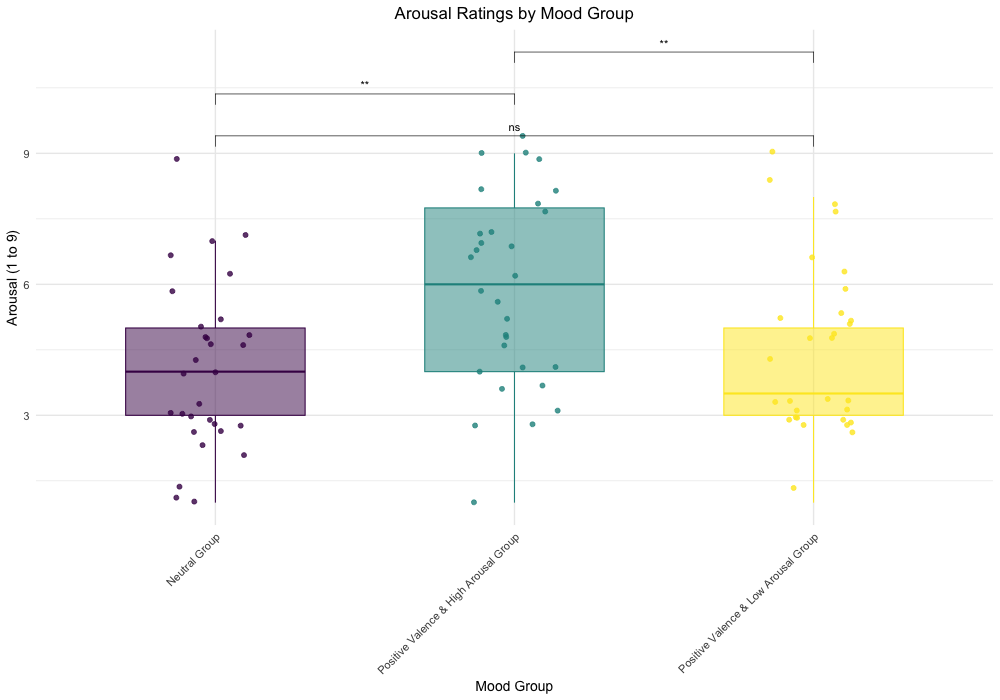
\includegraphics[width=\textwidth]{../analysis/results/main_results/mood_induction_check/arousal_by_group.png}
  \caption{Boxplot of Arousal Ratings by Mood Group}
  \label{fig:arousal_group}
\end{figure}

Valence was significantly different between groups, $F(2, 87) = 4.44$, $p = .0146$, revealing a moderate effect size ($\eta^2 = .09$). Post-hoc Tukey tests revealed that the \textit{High-Arousal Positive Mood} group ($M = 2.91$, $SD = 0.96$) reported significantly higher valence than the \textit{Neutral Control} group ($M = 1.24$, $SD = 1.24$; $p = .0167$), whereas the \textit{Low-Arousal Positive Mood} group ($M = 2.16$, $SD = 1.10$) did not significantly differ from either group ($ps > .05$; see Figure~\ref{fig:valence_group}). 

\begin{figure}[H]
  \centering
  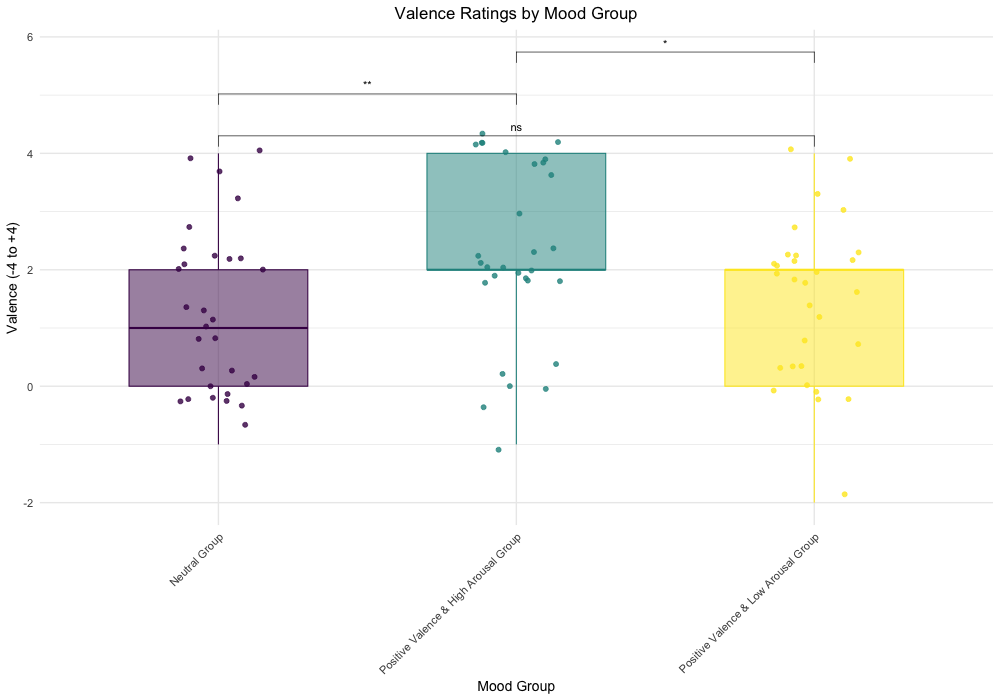
\includegraphics[width=\textwidth]{../analysis/results/main_results/mood_induction_check/valence_by_group.png}
  \caption{Boxplot of Valence Ratings by Mood Group}
  \label{fig:valence_group}
\end{figure}

Overall, the experimental mood induction procedure using three validated film clips achieved the anticipated mood manipulation results. For the two positive valence groups, there was a significant difference in arousal ratings, whereas the valence ratings did not significantly differ. This pattern supports the intended orthogonal manipulation of arousal while holding valence constant, allowing for a more focused investigation of arousal's unique effects on subsequent creative processes. Meanwhile, the significant differences in both arousal and valence ratings between the \textit{High-Arousal Positive Mood} and \textit{Neutral Control} groups confirm the successful induction of a distinctly activated positive affective state in the high-arousal condition.

\subsection*{Descriptive Statistics of Flexibility and Originality Measures}

The descriptive statistics for all the measures of flexibility and originality across mood conditions are presented in Table~\ref{tab:descriptive_stats}. Overall, the flexibility metrics demonstrated subtle group differences. Average entropy and Bhattacharyya distance were highest in \textit{High-Arousal Positive} group and lowest in \textit{Low-Arousal Positive} group, though these differences were small. Inflection proportions of entropy and Bhattacharyya distance were slightly elevated in \textit{Low-Arousal Positive} group, suggesting greater within-trial shifts in drawing strategy. DSI scores were highest in \textit{High- Arousal Positive} group, indicating more semantically diverse narrative content, with \textit{Neutral Control} and \textit{Low-Arousal Positive} groups showing similar levels. Originality, as measured by the AuDrA model, remained stable under all conditions, with means ranging narrowly from 0.36 to 0.37 and no apparent variation across groups. 

To further statistically assess group differences across the three induced mood conditions, a series of one-way ANOVAs were performed for each flexibility measure and originality. As shown in Table~\ref{tab:anova_results}, none of the ANOVAs reached significance and all effect sizes were small ($\eta^2 < .03$). This suggests that mood induction did not lead to significant differences in cognitive flexibility or originality. In other words, mood induction, despite being shown to alter the arousal and valence ratings, did not affect the originality aspect of creativity or any of the process measures, as mentioned in previous studies. 

\begin{table}[H]
\centering
\begin{threeparttable}
\caption{Descriptive Statistics by Mood Condition (Mean (SD))}
\label{tab:descriptive_stats}
\begin{tabular}{lccc}
\toprule
\textbf{Measure} & \textbf{Neutral Group} & \textbf{High Arousal Group} & \textbf{Low Arousal Group} \\
\midrule
Avg. Entropy & 1.77 (0.09) & 1.78 (0.07) & 1.74 (0.10) \\
Avg. Bhatt. Dist. & 2.51 (0.29) & 2.50 (0.25) & 2.45 (0.28) \\
Inflect. Prop. Entropy & 0.41 (0.18) & 0.42 (0.17) & 0.45 (0.17) \\
Inflect. Prop. Bhatt & 0.42 (0.18) & 0.43 (0.16) & 0.44 (0.20) \\
DSI & 0.59 (0.28) & 0.66 (0.22) & 0.58 (0.30) \\
AuDrA & 0.37 (0.10) & 0.36 (0.10) & 0.37 (0.11) \\
\bottomrule
\end{tabular}
\begin{tablenotes}[flushleft]
\small
\item \textit{Note.} Avg. Entropy = Average Entropy; Avg. Bhatt. Dist. = Average Bhattacharyya Distance; Inflect. Prop. Entropy = Inflection Proportion of Entropy; Inflect. Prop. Bhatt = Inflection Proportion of Bhattacharyya Distance; DSI = Divergent Semantic Integration; AuDrA = Automated Drawing Assessment (Originality Score).
\end{tablenotes}
\end{threeparttable}
\end{table}

\begin{table}[H]
\centering
\begin{threeparttable}
\caption{One-way ANOVA Results for Group Comparisons}
\label{tab:anova_results}
\begin{tabular}{lccc}
\toprule
\textbf{Measure} & \textbf{$F(2, 87)$} & \textbf{$p$} & \textbf{$\eta^2$} \\
\midrule
Avg. Entropy & 1.30 & .2784 & .029 \\
Avg. Bhatt. Dist. & 0.44 & .6456 & .010 \\
Inflect. Prop. Entropy & 0.41 & .6620 & .009 \\
Inflect. Prop. Bhatt & 0.12 & .8850 & .003 \\
DSI & 0.63 & .5375 & .014 \\
AuDrA & 0.18 & .8357 & .004 \\
\bottomrule
\end{tabular}
\begin{tablenotes}[flushleft]
\small
\item \textit{Note.} Avg. Entropy = Average Entropy; Avg. Bhatt. Dist. = Average Bhattacharyya Distance; Inflect. Prop. Entropy = Inflection Proportion of Entropy; Inflect. Prop. Bhatt = Inflection Proportion of Bhattacharyya Distance; DSI = Divergent Semantic Integration; AuDrA = Automated Drawing Assessment (Originality Score).
\end{tablenotes}
\end{threeparttable}
\end{table}

\subsection*{Correlational and Predictive Analyses of Flexibility Measures}

When it comes to the relationship between the process measures of creativity and the originality aspect of creativity, correlation analyses revealed a notable divergence between two modes of cognitive flexibility. As shown in Figure~\ref{fig:cor_heatmap}, average entropy and average Bhattacharyya distance were strongly positively correlated with each other ($r = .83$), but both showed insignificantly weak correlations with their respective inflection metrics and with DSI ($r$s between –.12 and –.18). These trends suggest that participants who sustained a broad space of exploratory stroke options throughout the drawing process tended to make fewer within-trial shifts in drawing strategy and produced less semantically divergent narratives.

\begin{figure}[H]
  \centering
  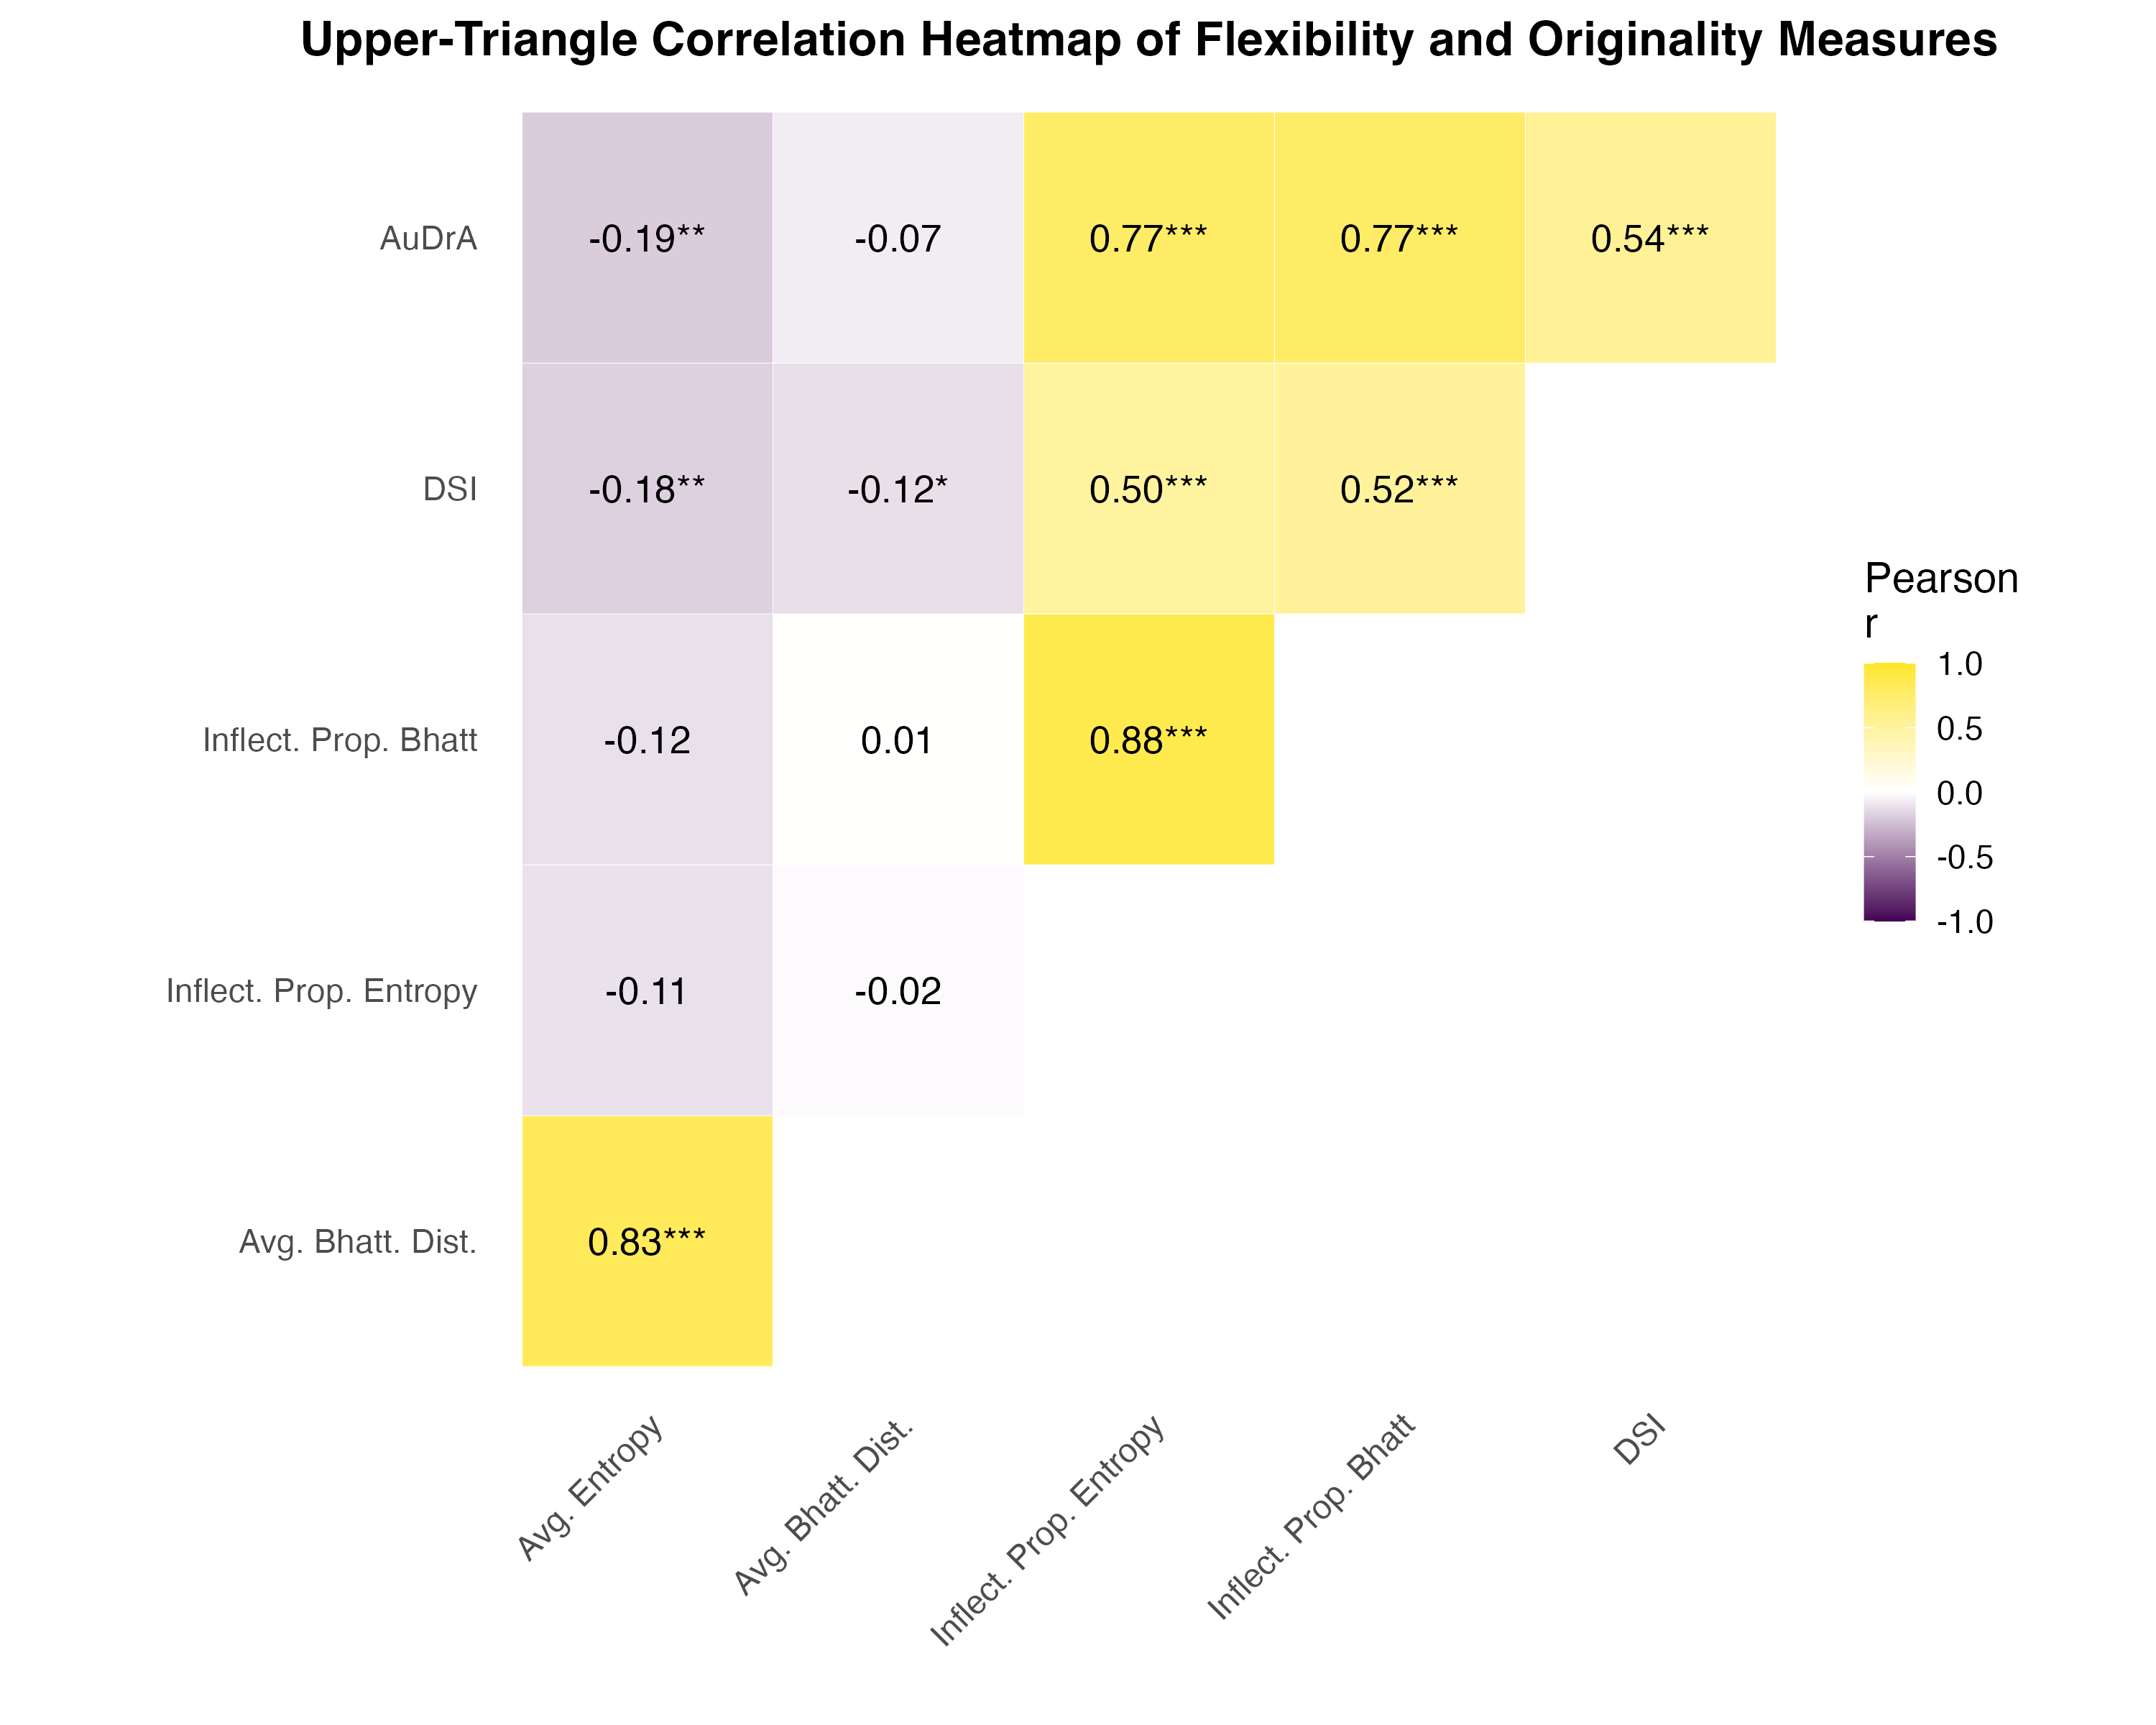
\includegraphics[width=\textwidth]{../analysis/results/main_results/correlation/correlation_heatmap.png}
  \caption{
    Pearson Correlation Heatmap of Flexbility and Originality Measures.
  }
  \label{fig:cor_heatmap}
\end{figure}

In contrast, the two inflection-based measures were strongly positively correlated with each other ($r = .88$), and both were moderately positively associated with DSI ($r > .50$), indicating a shared flexibility dynamic rooted in frequent strategic switching and a wider conceptual integration. These switching-based flexibility metrics demonstrated a modest positive relationship with originality (AuDrA), while the average metrics (entropy and Bhattacharyya distance) showed little to no association with originality.

Taken together, these results suggest that real-time flexibility may manifest through two distinct behavioral strategies: one characterized by persistent exploratory breadth (high average entropy and Bhattacharyya distance) and another characterized by dynamic switching between ideas (high inflection proportions and DSI). Importantly, only the latter appears to be meaningfully connected to originality in this task context.

\subsubsection*{Multilevel Regression Analysis: Direct Prediction of Originality}
Given that mood induction did not significantly influence originality or any flexibility process measures (as established through the series of one-way ANOVAs above), one of the necessary conditions for the mediation analysis (i.e., the significance of both the indirect and direct effects) was not met. Hence, we chose not to perform the planned mediation analysis (see the full mediation model output in Appendix~\ref{appendix: mediation_analysis_results} that confirms the insignificance of indirect and direct effects of positive, activating mood states on originality). Despite the failure of replication of the hypothesized flexibility pathway linking positive, activating mood states to originality in previous studies, 

\end{document}